\chapter{Perancangan}
\label{chap:perancangan}

Perancangan yang dibuat pada bab ini meliputi tiga perangkat lunak yaitu eksplorasi, anonimisasi, dan pengujian. Pada perangkat lunak eksplorasi akan dilakukan pencarian nilai unik untuk setiap atribut. Pada perangkat lunak anonimisasi akan dilakukan pemodelan algoritma greedy k-member clustering dan k-anonymity. Pada perangkat lunak pengujian akan dilakukan pemodelan k-means dan naive bayes. Pada tahap ini tidak dilakukan perancangan terhadap tampilan antarmuka karena program yang dihasilkan akan dijalankan dengan menggunakan command prompt.

\begin{figure}[H]
	\centering
	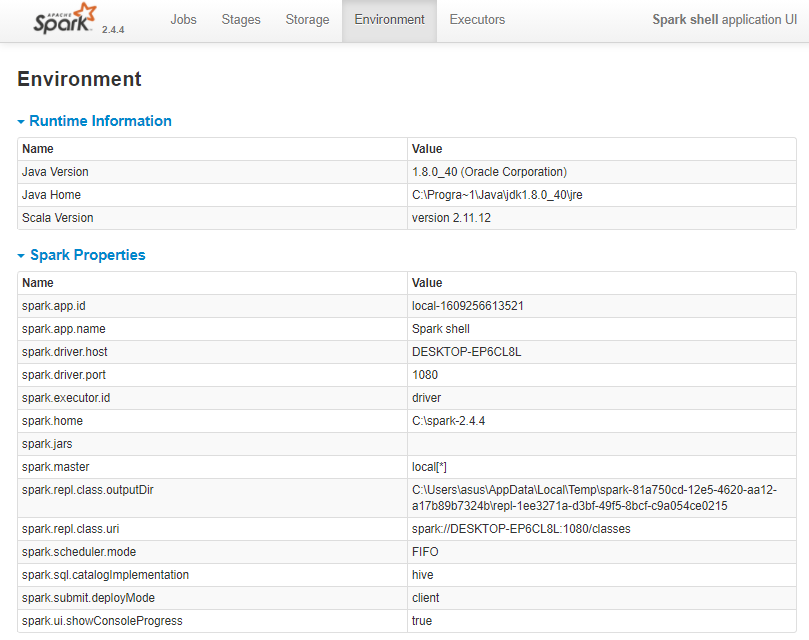
\includegraphics[scale=0.6]{bab4_antarmuka1.PNG}
	\caption{Flow Chart Penggunaaan Perangkat Lunak}
	\label{fig:diagram_aktivitas_bab4}
\end{figure}

\begin{figure}[H]
	\centering
	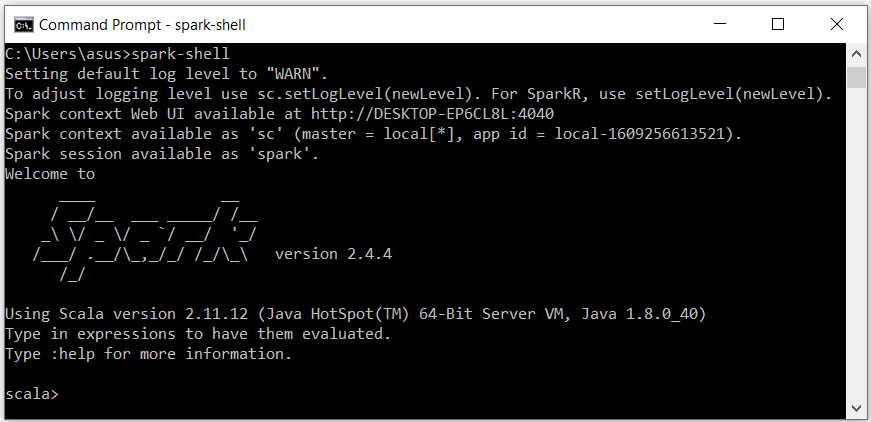
\includegraphics[scale=0.6]{bab4_antarmuka2.PNG}
	\caption{Flow Chart Penggunaaan Perangkat Lunak}
	\label{fig:diagram_aktivitas_bab4}
\end{figure}


\newpage
\section{Diagram Kelas Lengkap}
\label{sec:diagram_kelas_lengkap}

Pada bagian ini, akan dibuat empat jenis diagram kelas, yaitu diagram kelas untuk package, diagram kelas untuk perangkat lunak eksplorasi, diagram kelas untuk perangkat lunak anonimisasi, dan diagram kelas untuk perangkat lunak pengujian.

\subsection{Diagram Package}
\label{sec:perangkat_lunak_anonimisasi}

Perangkat lunak ini mempunyai 3 buah package yang tidak saling berhubungan satu sama lain yaitu ExploratoryModel, AnonymizationModel, ExaminationModel. Ketika package ini memiliki fungsinya masing-masing. Diagram Package dapat dilihat pada Gambar \ref{fig:dc_package_model}

\begin{figure}[H]
	\centering
	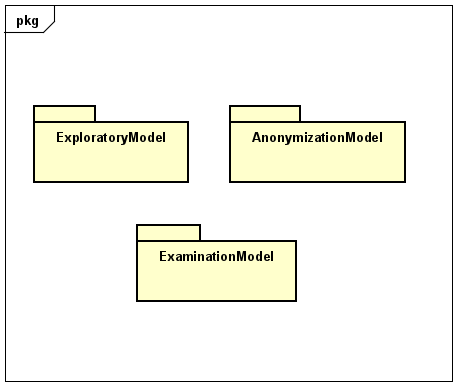
\includegraphics[scale=1]{dc_package_model}
	\caption{Diagram Kelas pada Package}
	\label{fig:dc_package_model}
\end{figure}

\subsubsection{Package ExploratoryModel}
Package ExploratoryModel merupakan package yang menangani pencarian nilai unik pada masing-masing atribut. Package ini hanya memiliki implementasi kelas Main untuk mencari nilai atribut yang unik dan mengembalikan nilai unik tersebut ke dalam tabel data yang disimpan dalam format CSV. Jumlah CSV yang dihasilkan bergantung pada jumlah atribut yang dicantumkan pada JSON.

\subsubsection{Package AnonymizationModel}
Package AnonymizationModel merupakan package yang menangani segala jenis fungsi yang berkaitan dengan masalah pengelompokan data dan anonimisasi data. Fungsi tersebut antara lain pengelompokan data dengan algoritma Greedy k-member clustering, pencarian record dan cluster terbaik, perhitungan distance numerik dan kategorikal, dan perhitungan information loss. Package ini juga mengimplementasikan berbagai macam operasi untuk membaca atribut DGH pada JSON dan menangani pembuatan binary tree berdasarkan atribut DGH. Operasi-operasi ini diimplementasikan karena adanya kebutuhan untuk membantu proses implementasi pengelompokan data dan anonimisasi data. Selain itu, package ini memiliki dua jenis kelas Main yaitu MainTesting dan MainLCATesting. Kelas MainTesting digunakan untuk melakukan proses pengelompokan dan anonimisasi data dan mengembalikan hasilnya ke dalam format CSV. Kelas MainLCATesting digunakan untuk menampilkan root terdekat dari kedua node. 

\subsubsection{Package ExaminationModel}
Package ExaminationModel merupakan package yang menangani segala jenis fungsi yang berkaitan dengan masalah pengujian data. Fungsi tersebut antara lain pengelompokan data dengan pemodelan k-means beserta evaluasi modelnya dengan silhouette score dan pemodelan naive bayes beserta evaluasi modelnya dengan accuracy. Package ini juga mengimplementasikan berbagai macam operasi untuk membuat DataFrame berdasarkan atribut yang telah dipilih pada JSON dan mendapatkan nilai parameter k-means dan naive bayes dari JSON. Operasi-operasi ini diimplementasikan karena adanya kebutuhan untuk membantu proses pengujian data berdasarkan pemodelan yang dipilih (k-means/naive bayes). Selain itu, package ini memiliki satu jenis kelas Main yaitu MainTesting. Kelas MainTesting digunakan untuk melakukan pengujian data dengan pemodelan k-means/naive bayes dan mengembalikan hasilnya ke dalam format CSV.


\subsection{Diagram Kelas pada Package ExploratoryModel}

\noindent Perangkat lunak eksplorasi hanya memiliki satu jenis \textit{package} dengan nama \textit{ExploratoryModel}. \textit{Package ExploratoryModel} terdiri dari satu kelas yaitu MainTesting. Kelas ini memiliki fungsi penting untuk menyelesaikan permasalahan pencarian nilai atribut yang unik.

\begin{figure}[H]
	\centering
	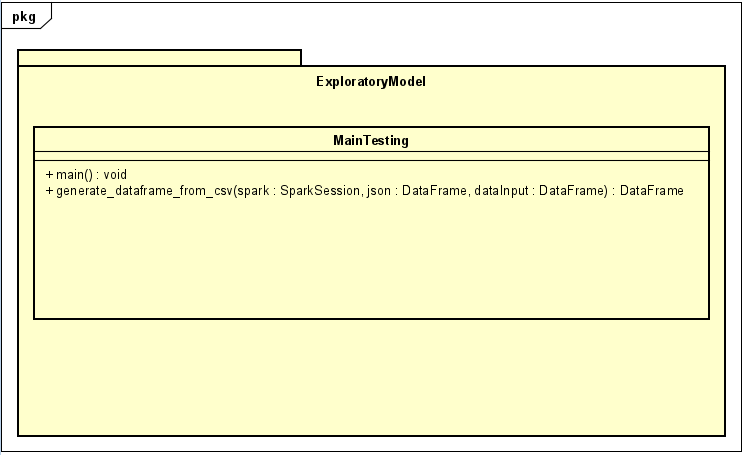
\includegraphics[scale=0.8]{dc_exploratory_model}
	\caption{Diagram Kelas pada Package ExploratoryModel}
	\label{fig:dc_exploratory_model}
\end{figure}

\subsubsection{Kelas \textit{MainTesting}}
Kelas \textit{MainTesting} merupakan kelas dengan tipe \textit{object}, karena kelas ini memiliki method Main untuk menjalankan eksekusi program. Kelas ini berperan penting untuk mencari nilai unik setiap atribut. Hasil eksekusi kelas ini akan menghasilkan output berupa beberapa jenis CSV yang bergantung kepada jumlah atribut yang ingin diketahui nilai uniknya dan atribut tersebut telah dicantumkan pada format JSON. Perlu diketahui bahwa kelas ini tidak memiliki atribut dan hanya memiliki sebuah method dengan nama \texttt{generate\_dataframe\_from\_csv} untuk membuat DataFrame berdasarkan atribut yang dipilih dan telah dicantumkan dalam format JSON.



\subsection{Diagram Kelas pada Package AnonymizationModel}

\noindent Perangkat lunak anonimisasi hanya memiliki satu jenis \textit{package}  bernama \textit{AnonymizationModel}. \textit{Package AnonymizationModel} terdiri dari beberapa kelas. Masing-masing kelas memiliki fungsi penting menyelesaikan permasalahan pengelompokan dan anonimisasi data.

\begin{figure}[H]
	\centering
	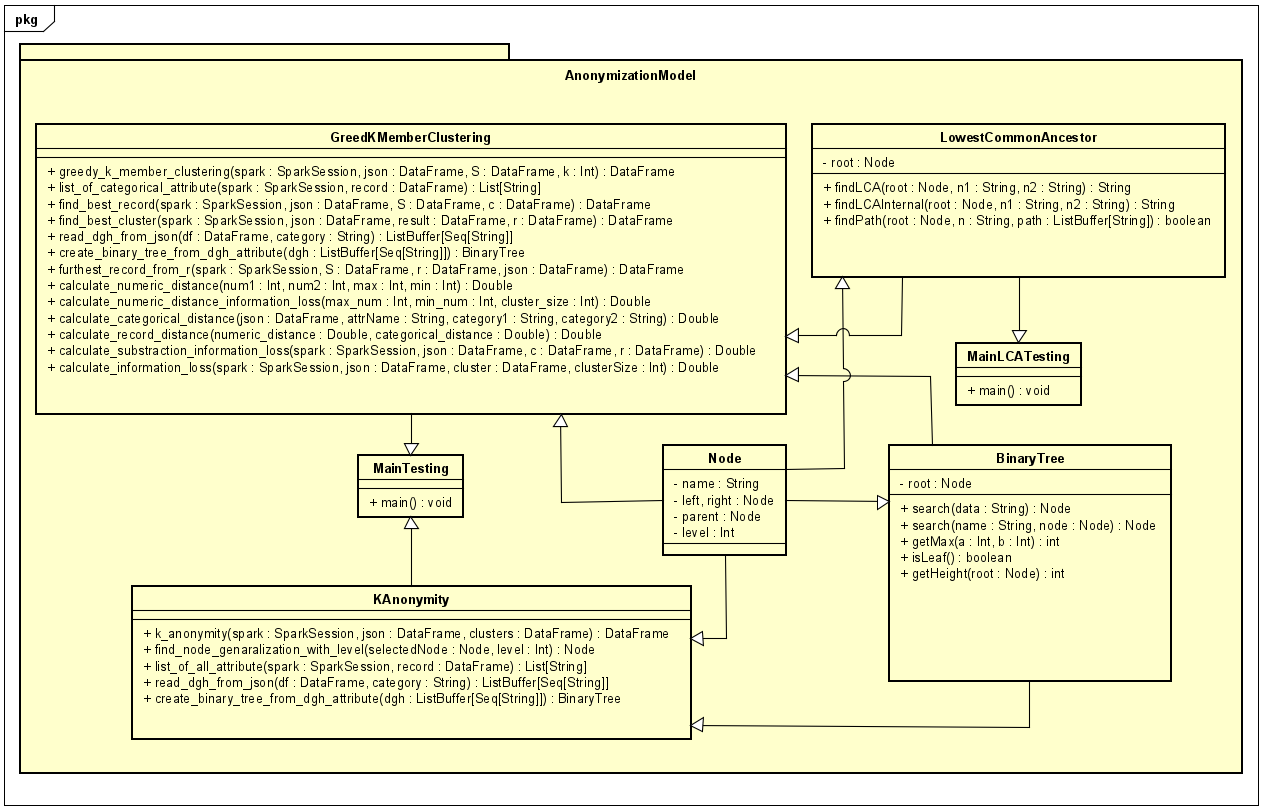
\includegraphics[scale=0.62]{dc_anonymization_model}
	\caption{Diagram Kelas pada Package AnonymizationModel}
	\label{fig:dc_anonymization_model}
\end{figure}

\subsubsection{Kelas \textit{Node}}
Kelas \textit{Node} merupakan kelas dengan tipe \textit{class}, karena kelas ini berfungsi sebagai model untuk membuat atribut dan \textit{method} pada objek \textit{Node}. Kelas ini bertujuan untuk menyimpan informasi seperti nama \textit{node}, menyatakan \textit{node} kiri dan \textit{node} kanan dari \textit{node} tersebut, menyatakan \textit{parent} dari \textit{node} tersebut, dan \textit{level} yang menyatakan posisi ketinggian \textit{node} pada objek \textit{BinaryTree}. Kelas \textit{Node} nantinya akan dipakai untuk pembuatan objek \textit{BinaryTree}.\\

\noindent Berikut adalah penjelasan masing-masing atribut pada kelas \textit{Node}:

\begin{itemize}

\item \texttt{name} adalah variabel yang berfungsi untuk menyimpan nilai atribut tertentu pada sebuah tabel data dengan tipe String dan termasuk jenis variabel \texttt{var} sehingga atribut ini nilainya bersifat \textit{mutable}/dapat diubah sesuai kebutuhan.

\item \texttt{left} adalah variabel yang berfungsi untuk menyimpan node kiri dari  node tersebut dengan tipe Node dan termasuk jenis variabel \texttt{var} sehingga atribut ini nilainya bersifat \textit{mutable}/dapat diubah sesuai kebutuhan.

\item \texttt{right} adalah variabel yang berfungsi untuk menyimpan node kanan dari node tersebut dengan tipe Node dan termasuk jenis variabel \texttt{var} sehingga atribut ini nilainya bersifat \textit{mutable}/dapat diubah sesuai kebutuhan.

\item \texttt{parent} adalah variabel yang berfungsi untuk menyimpan node \texttt{parent} dari node tersebut dengan tipe Node dan termasuk jenis variabel \texttt{var} sehingga atribut ini nilainya bersifat \textit{mutable}/dapat diubah sesuai kebutuhan.


\item \texttt{level} adalah variabel yang berfungsi untuk menyimpan posisi ketinggian BinaryTree untuk node tersebut dengan tipe Integer dan termasuk jenis variabel \texttt{var} sehingga atribut ini nilainya bersifat \textit{mutable}/dapat diubah sesuai kebutuhan.

\end{itemize}

\newpage
\subsubsection{Kelas \textit{BinaryTree}}
Kelas \textit{BinaryTree} merupakan kelas dengan tipe \textit{class}, karena kelas ini berfungsi sebagai model untuk membuat atribut dan method pada objek \textit{BinaryTree}. Kelas ini nantinya akan dipakai untuk pembuatan objek \textit{BinaryTree} berdasarkan \textit{Domain Generalization Hierarchy} (DGH).\\

\noindent  Berikut deskripsi atribut pada kelas \textit{BinaryTree}:

\begin{itemize}

\item \texttt{root} adalah variabel yang berfungsi untuk menyimpan node yang menjadi root pada objek BinaryTree dengan tipe Node dan termasuk jenis variabel \textit{var} sehingga atribut \textit{root} nilainya bersifat \textit{mutable}/dapat diubah sesuai kebutuhan.

\end{itemize}

\noindent  Berikut deskripsi atribut pada kelas \textit{BinaryTree}:

\begin{itemize}

\item \texttt{search} dengan parameter \texttt{data(String)} adalah fungsi yang akan memanggil fungsi search lain dengan parameter \textit{name(String)}, \textit{node(Node)} untuk mengembalikan objek \textit{Node} yang ingin dicari pada objek \textit{BinaryTree}.

\item \texttt{search} dengan parameter \texttt{name(String)}, \textit{node(Node)} adalah fungsi yang bertujuan untuk mengembalikan objek \textit{Node} yang ingin dicari pada objek \textit{BinaryTree}.

\item \texttt{getMax} dengan parameter \texttt{a(Integer)}, \texttt{b(Integer)} adalah fungsi yang bertujuan untuk mengembalikan nilai \textit{Integer} paling besar antara parameter \texttt{a} dan \texttt{b}.

\item \texttt{isLeaf} tanpa parameter adalah fungsi yang bertujuan untuk mengembalikan nilai \textit{Boolean} untuk menyatakan apakah root dari node kiri dan kanan bernilai \textit{null}. Jika kondisi terpenuhi maka nilainya \textit{true}, apabila tidak terpenuhi maka nilainya \textit{false}.

\item \texttt{getHeight} dengan parameter \texttt{root(Node)} adalah fungsi yang bertujuan untuk mengembalikan nilai \textit{Integer} untuk menyatakan ketinggian dari objek BinaryTree.

\end{itemize}

\noindent Berikut implementasi method \texttt{search} pada kelas \textit{BinaryTree}:

\begin{minipage}{.8\linewidth}
\begin{algorithm}[H]
  \caption{Mencari Node dengan Nama Tertentu}\label{alg:4}
  \begin{algorithmic}[1]
  %-------------- Input & Output -----------------
  \State \textbf{Function} \texttt{search(name,node)}
  \State \textbf{Input:} a name of node (name) and a node.
  \State \textbf{Output:} a node with selected name.
  \\
  %-------------- Baris 1-3 -----------------
  \If{node != null}
  	\If{node.name == name}
  		\State{return node}
  	\Else 
  		\State{$foundNode = search(name,node.left)$}
  		\If{foundNode == null}
  			\State{$foundNode = search(name,node.right)$}
  		\EndIf
  		\State{return foundNode}
  	\EndIf
  \Else 
  	\State{return null}
  \EndIf
  \end{algorithmic}
\end{algorithm}
\end{minipage}

\vspace{0.2cm}
\begin{itemize}
\item Baris 6-8: baris ini mengembalikan sebuah node, jika nama sebuah node sudah sesuai.
\item Baris 9-14: baris ini melakukan proses rekursif untuk mencari nama node yang sesuai.
\end{itemize}

\newpage
\subsubsection{Kelas \textit{LowestCommonAncestor}}
Kelas \textit{LowestCommonAncestor} merupakan kelas dengan tipe \textit{class}. Hal ini dikarenakan kelas \textit{LowestCommonAncestor} berfungsi sebagai model untuk membuat atribut dan method-method pada objek \textit{LowestCommonAncestor}. Kelas \textit{LowestCommonAncestor} bertujuan untuk melakukan pencarian node root terdekat dari kedua node. Kelas \textit{LowestCommonAncestor} nantinya akan dipakai untuk mencari level node root terdekat untuk menghitung distance kategorikal.\\

\noindent Berikut deskripsi atribut pada kelas \textit{LowestCommonAncestor}:

\begin{itemize}

\item \texttt{path1} adalah variabel yang berfungsi untuk menyimpan list node yang pernah dipilih sebelumnya dengan tipe ListBuffer[String] dan termasuk jenis variabel \textit{var} sehingga atribut \textit{path1} nilainya bersifat \textit{mutable}/dapat diubah sesuai kebutuhan.

\item \texttt{path2} adalah variabel yang berfungsi untuk menyimpan list node yang pernah dipilih sebelumnya dengan tipe ListBuffer[String] dan termasuk jenis variabel \textit{var} sehingga atribut \textit{path1} nilainya bersifat \textit{mutable}/dapat diubah sesuai kebutuhan.

\end{itemize}

\noindent Berikut deskripsi method pada kelas \textit{LowestCommonAncestor}:

\begin{itemize}

\item \texttt{findLCA} dengan parameter \texttt{root(Node)}, \texttt{n1(String)}, \textit{n2(String)} adalah fungsi yang bertujuan untuk mereset nilai path1 dan path2 dan memanggil fungsi \texttt{findLCAInternal} untuk mencari nama root paling bawah yang mengandung kedua node.

\item \texttt{findLCAInternal} dengan parameter \textit{root(Node)}, \texttt{n1(String)}, \texttt{n2(String)} adalah fungsi yang bertujuan untuk mencari nama root paling bawah yang mengandung kedua node. Caranya dengan menambahkan indeks pada setiap iterasi, jika nama node pada path1 sama dengan nama node pada path2. Indeks ini nantinya dipakai untuk mengambil nama node pada path1 sebagai hasil output dari algoritma Lowest Common Ancestor.

\item \texttt{findPath} dengan parameter \textit{root(Node)}, \textit{n(String)}, \textit{path(ListBuffer[String])} adalah fungsi yang bertujuan untuk menambahkan node yang pernah diproses sebelumnya pada method ini sebagai elemen untuk array \texttt{path 1} dan \texttt{path 2}. Method ini akan mengembalikan nilai true, jika nama node yang diberikan sama dengan nama yang dicari.

\end{itemize}

\noindent Berikut implementasi method \texttt{findLCAInternal} pada kelas \textit{LowestCommonAncestor}:

\begin{minipage}{.8\linewidth}
\begin{algorithm}[H]
  \caption{Mencari Nama Root Terdekat dengan Kedua Node}\label{alg:5}
  \begin{algorithmic}[1]
  %-------------- Input & Output -----------------
  \State \textbf{Function} \texttt{findLCAInternal(root,namenode1,namenode2)}
  \State \textbf{Input:} root node (root), name of node 1 (n1), name of node 2 (n2).
  \State \textbf{Output:} a name of root node.
  \\
  %-------------- Baris 1-3 -----------------
  \If{(!findPath(root,namenode1,path1) or !findPath(root,namenode2,path2))}
  	\State{return "not found"}
  \EndIf
  \\
  \State{$i = 0$}
  \\
  \While {(i < path1.size and i < path2.size)}
  	\If{!path1(i).equals(path2(i))}
  		\State{$i += 1$}
  	\EndIf
  \EndWhile
  \State{return path1(i-1)}
  \end{algorithmic}
\end{algorithm}
\end{minipage}

\vspace{0.2cm}
\begin{itemize}
\item Baris 5-7: baris ini memeriksa apakah nama node 1 dan nama node 2 ada pada objek Binary Tree, jika tersedia maka method akan mengembalikan nilai true.
\item Baris 9: baris ini digunakan untuk mengambil nama node yang pernah dikunjungi sebelumnya pada indeks ke-i dari elemen array pada \texttt{path1} dan elemen array pada \texttt{path2}.
\item Baris 11-15: baris ini melakukan perulangan untuk mencari nama node root paling rendah, dengan objek node 1 dan node 2 sebagai anak dari node root tersebut. 
\item Baris 12-14: baris ini mencari nama root terdekat dengan menambahkan indeks pada setiap iterasi, jika node 1 memiliki nama yang sama dengan node 2.
\item Baris 16: pada baris ini, iterasi yang diperoleh akan dipakai untuk menyatakan nama dari node root terdekat antara node 1 dan node 2.
\end{itemize}

\noindent Berikut implementasi method \texttt{findPath} pada kelas \textit{LowestCommonAncestor}:

\begin{minipage}{.8\linewidth}
\begin{algorithm}[H]
  \caption{Mencari Node yang Pernah Dilalui Sebelumnya}\label{alg:6}
  \begin{algorithmic}[1]
  %-------------- Input & Output -----------------
  \State \textbf{Function} \texttt{findPath(root,namenode,path)}
  \State \textbf{Input:} root node (root), name of node (n), path of node.
  \State \textbf{Output:} true/false.
  \\
  %-------------- Baris 1-3 -----------------
  \If{(root == null)}
  	\State{return false}
  \EndIf
  \State{$path += root.name$}
  \\
  \If{(root.name == namenode)}
  	\State{return true}
  \EndIf
  \\
  \If{(root.left != null and findPath(root.left, n, path))}
  	\State{return true}
  \EndIf
  \\
  \If{(root.right != null and findPath(root.right, n, path))}
  	\State{return true}
  \EndIf
  \State{path.remove(path.size - 1)}
  \State{return false}
  \end{algorithmic}
\end{algorithm}
\end{minipage}

\vspace{0.2cm}
\begin{itemize}
\item Baris 5-7: baris ini akan mengembalikan nilai \textit{false} jika \textit{node} sudah kosong.
\item Baris 9: baris ini akan mencatat setiap \textit{node} yang pernah dikunjungi ke dalam variabel \texttt{path}
\item Baris 11-13: baris ini akan mengembalikan nilai \textit{true} jika node yang dikunjungi memiliki nama yang sama dengan nama yang ingin dicari 
\item Baris 15-17: baris ini akan memeriksa apakah setiap \textit{node} kiri dari sebuah node memiliki nama yang dicari, jika benar maka akan mengembalikan nilai \textit{true}.
\item Baris 19-21: baris ini akan memeriksa apakah setiap \textit{node} kanan dari sebuah \textit{node} memiliki nama yang dicari, jika benar maka akan mengembalikan nilai \textit{true}.
\item Baris 23: setiap kali method ini dipanggil, maka \textit{node} paling terakhir akan dihapus dari kumpulan node yang sudah pernah dicatat sebelumnya pada variabel \texttt{path}.
\end{itemize}


\subsubsection{Kelas \textit{GreedyKMemberClustering}}
Kelas \textit{GreedyKMemberClustering} merupakan kelas dengan tipe \textit{class}. Hal ini dikarenakan kelas \textit{GreedyKMemberClustering} berfungsi sebagai model untuk membuat atribut dan method pada objek \textit{GreedyKMemberClustering}. Kelas \textit{GreedyKMemberClustering} bertujuan untuk melakukan fungsi pengelompokan data. Kelas \textit{GreedyKMemberClustering} tidak memiliki atribut.\\

\noindent Berikut deskripsi method pada kelas \textit{GreedyKMemberClustering}:

\begin{itemize}

\item \texttt{greedy\_k\_member\_clustering} dengan parameter \texttt{spark(SparkSession)}, \texttt{json(DataFrame)}, \texttt{S(DataFrame)}, \texttt{k(Integer)} adalah fungsi yang bertujuan untuk melakukan pengelompokan data dengan algoritma Greedy k-member clustering sebelum data dilakukan anonimisasi. Kelompok data yang terbentuk akan didasari pada selisih information loss paling minimum antar masing-masing data berdasarkan fungsi \texttt{find\_best\_record} dan fungsi \texttt{find\_best\_cluster}.

\item \texttt{list\_of\_categorical\_attribute} dengan parameter \texttt{spark(SparkSession}, \texttt{record (Data Frame)} adalah fungsi yang bertujuan untuk mendapatkan seluruh nama atribut dari tabel data. Fungsi lain seperti \texttt{furthest\_record\_from\_r}, \texttt{calculate\_information\_loss} akan memanggil fungsi ini untuk mendapatkan tabel data yang berisi kolom-kolom bertipe kategorikal, sebelum tabel data dipakai untuk mencari record paling jauh dengan record r dan sebelum tabel data dipakai untuk menghitung nilai information loss pada kelompok data.

\item \texttt{find\_best\_record} dengan parameter \texttt{spark(SparkSession)}, \texttt{json(DataFrame)}, \texttt{S(Data Frame)}, \texttt{c(DataFrame)} adalah fungsi yang bertujuan untuk mencari setiap record dari tabel data yang memiliki nilai information loss paling minimum terhadap record c.

\item \texttt{find\_best\_cluster} dengan parameter \texttt{spark(SparkSession)}, \texttt{json(DataFrame)}, \texttt{S (Data Frame)}, \texttt{r(DataFrame)} adalah fungsi yang bertujuan untuk mencari setiap record dari tabel data yang telah dikelompokan dengan nilai information loss paling rendah terhadap sebuah record r, dimana r adalah record yang belum masuk kelompok data tertentu.

\item \texttt{read\_dgh\_from\_json} dengan parameter \texttt{df(DataFrame)}, \texttt{category(String)} adalah fungsi yang bertujuan untuk mengembalikan nilai \texttt{value,parent,level,position} untuk setiap nama atribut tabel data pada \texttt{domain\_generaliation\_hierarchy} JSON.

\item \texttt{create\_binary\_tree\_from\_dgh\_attribute} dengan parameter \texttt{dgh(ListBuffer[Seq[String ]])}, \texttt{category(String)} adalah fungsi yang bertujuan untuk membuat pohon DGH melalui representasi objek BinaryTree pada \texttt{domain\_generaliation\_hierarchy} JSON.

\item \texttt{furthest\_record\_from\_r} dengan parameter \texttt{spark(SparkSession)}, \texttt{S(DataFrame)}, \texttt{r (Data Frame)}, \texttt{json(DataFrame)} adalah fungsi yang bertujuan untuk menghitung distance record antara record r dengan masing-masing record pada tabel data. Setelah dilakukan perhitungan, record dengan nilai distance record tertinggi akan dikembalikan sebagai output dari fungsi ini.

\item \texttt{calculate\_numeric\_distance} dengan parameter \texttt{num1(Int)}, \texttt{num2(Int)}, \texttt{max(Int)}, \texttt{min(Int )} adalah fungsi yang bertujuan untuk menghitung distance numerik antara 2 data numerik dengan atribut yang sejenis. Fungsi ini dipanggil oleh fungsi lain yaitu \texttt{furthest\_record\_from\_r}, agar hasil perhitungan distance numerik dapat digunakan untuk menghitung distance record.

\item \texttt{calculate\_numeric\_distance\_information\_loss} dengan parameter \texttt{max\_num(Integer)}, \texttt{min\_num(Integer)}, \texttt{cluster\_size(Integer)} adalah fungsi yang bertujuan untuk menghitung distance numerik pada kasus information loss antar 2 data numerik di atribut yang sejenis. Fungsi ini dipanggil oleh fungsi lain yaitu \texttt{calculate\_information\_loss}, agar hasil perhitungan distance numerik dapat digunakan untuk menghitung nilai information loss pada sebuah kelompok data untuk mendapatkan hasil pengelompokan data yang terbaik.

\newpage
\item \texttt{calculate\_categorical\_distance} dengan parameter \texttt{json(DataFrame)},\texttt{attrName(String)}, \texttt{category1(String)}, \texttt{category1(String)} adalah fungsi yang bertujuan untuk menghitung distance kategorikal antara 2 data kategori dengan atribut yang sejenis. Fungsi ini dipanggil oleh fungsi \texttt{furthest\_record\_from\_r} untuk menghitung distance record.

\item \texttt{calculate\_record\_distance} dengan parameter \texttt{numeric\_distance(Double)}, \texttt{categorical\_ distance (Double)} adalah fungsi yang bertujuan untuk menghitung distance record antara 2 record. Fungsi ini dipanggil oleh fungsi \texttt{furthest\_record\_from\_r} untuk mencari record dengan distance record paling kecil. Distance record didapat dengan menjumlahkan total distance numerik dan total distance kategorikal.

\item \texttt{calculate\_substraction\_information\_loss} dengan parameter  \texttt{spark (SparkSession)}, \\ \texttt{json(DataFrame)}, \texttt{c(DataFrame)}, \texttt{r(DataFrame)} adalah fungsi yang bertujuan untuk mencari selisih information loss antara dua kelompok tabel data yang berbeda. Fungsi ini dipanggil oleh fungsi lain seperti \texttt{find\_best\_record} dan \texttt{find\_best\_cluster} untuk mencari record terbaik berdasarkan selisih  information loss paling kecil.

\item \texttt{calculate\_information\_loss} dengan parameter \texttt{spark(SparkSession)}, \texttt{json(DataFrame)}, \texttt{cluster(DataFrame)}, \texttt{clusterSize(Integer)} adalah fungsi yang bertujuan untuk menghitung nilai information loss pada kelompok tabel data tertentu. Fungsi ini dipanggil oleh fungsi lain seperti \texttt{calculate\_substraction\_information\_loss} untuk mencari selisih information loss antara dua kelompok tabel data yang berbeda.

\end{itemize}

\noindent Berikut implementasi method \texttt{calculate\_categorical\_distance}:

\begin{minipage}{.85\linewidth}
\begin{algorithm}[H]
  \caption{Menghitung Distance Kategorikal}\label{alg:6}
  \begin{algorithmic}[1]
  %-------------- Input & Output -----------------
  \State \textbf{Function} \texttt{calculate\_categorical\_distance(json,attrName,cat1,cat2)}
  \State \textbf{Input:} numeric 1, numeric 2, maximum number, maximum number.
  \State \textbf{Output:} numeric distance.
  \\
  %-------------- Baris 1-3 -----------------
  \State{result = 0.0}
  \State{dgh = read\_dgh\_from\_json(json, attrName)}
  \\
  \If{(dgh == null)}
 	 \State{return result}
  \EndIf
  \\
  \State{binaryTree = create\_binary\_tree\_from\_dgh\_attribute(dgh)}
  \State{node1 = binaryTree.search(category1)}
  \State{node2 = binaryTree.search(category2)}
  \\
  \If{(node1 != null and node2 != null)}
 	 \State{LCA = new LowestCommonAncestor()}
 	 \State{resultLCA = LCA.findLCA(binaryTree.root, node1.name, node2.name)}
 	 \State{H\_subtree = binaryTree.search(resultLCA).level}
 	 \State{H\_TD = binaryTree.getHeight(binaryTree.root).toDouble}
 	 \State{result = H\_subtree / H\_TD}
  \EndIf
  \\
  \State{result = BigDecimal(result)}
  \State{result = result.setScale(2, BigDecimal.RoundingMode.HALF\_UP)}  
  \State{result = result.toDouble}
  \State{return result}
  \end{algorithmic}
\end{algorithm}
\end{minipage}

\vspace{0.2cm}
\begin{itemize}
\item Baris 6: baris ini mendapatkan nilai \texttt{value,parent,level,position} untuk setiap nama atribut pada \texttt{domain\_generalization\_hierarchy} JSON.
\item Baris 8-10: baris ini memeriksa jika nilai pada \texttt{domain\_generalization\_hierarch} JSON kosong, maka perhitungan distance kategorikal tidak perlu dilakukan.
\item Baris 12: baris ini membuat objek BinaryTree berdasarkan atribut \texttt{dgh} pada baris 6.
\item Baris 13: baris ini mendapatkan objek Node pertama dengan parameter nama tertentu.
\item Baris 14: baris ini mendapatkan objek Node kedua dengan parameter nama tertentu.
\item Baris 16-22: baris ini menghitung \textit{distance} kategorikal jika kedua node tidak kosong.
\item Baris 19: baris ini menyimpan ketinggian \texttt{node root} dari objek \texttt{LowestCommonAncestor}
\item Baris 20: baris ini menyimpan ketinggian maksimal dari objek \texttt{BinaryTree}
\item Baris 24-26: baris ini mengembalikan hasil perhitungan \textit{distance}kategorikal dalam format desimal, dengan ketelitian 2 angka dibelakang koma.
\end{itemize}


\noindent Berikut implementasi method \texttt{calculate\_numeric\_distance}:

\begin{minipage}{.85\linewidth}
\begin{algorithm}[H]
  \caption{Menghitung Distance Numerik}\label{alg:6}
  \begin{algorithmic}[1]
  %-------------- Input & Output -----------------
  \State \textbf{Function} \texttt{calculate\_numeric\_distance(num1,num2,max,min)}
  \State \textbf{Input:} numeric 1, numeric 2, maximum number, maximum number.
  \State \textbf{Output:} numeric distance.
  \\
  %-------------- Baris 1-3 -----------------
  \State{v1 = num1}
  \State{v2 = num1}
  \State{diff = Math.abs(v1-v2)}
  \State{range = Math.abs(max-min)}
  \State{result = diff/range}
  \State{return result}
  \end{algorithmic}
\end{algorithm}
\end{minipage}

\vspace{0.2cm}
\begin{itemize}
\item Baris 5: baris ini melakukan inisialisasi \texttt{v1} dengan nilai \texttt{num1}.
\item Baris 6: baris ini melakukan inisialisasi \texttt{v2} dengan nilai \texttt{num2}.
\item Baris 7: baris ini menghitung selisih perbedaan nilai antara \texttt{v1} dan \texttt{v2}.
\item Baris 8: baris ini menghitung selisih range nilai antara \texttt{v1} dan \texttt{v2}.
\item Baris 9: baris ini membagi selisih perbedaan nilai dengan selisih \textit{range} nilai.
\end{itemize}


\noindent Berikut implementasi method \texttt{calculate\_record\_distance}:

\begin{minipage}{.85\linewidth}
\begin{algorithm}[H]
  \caption{Menghitung Distance Record}\label{alg:6}
  \begin{algorithmic}[1]
  %-------------- Input & Output -----------------
  \State \textbf{Function} \texttt{calculate\_record\_distance(num\_dist,cat\_dist)}
  \State \textbf{Input:} numeric 1, numeric 2, maximum number, maximum number.
  \State \textbf{Output:} numeric distance.
  \\
  %-------------- Baris 1-3 -----------------
  \State{result = numeric\_distance+categorical\_distance}
  \State{return result}
  \end{algorithmic}
\end{algorithm}
\end{minipage}

\vspace{0.2cm}
\begin{itemize}
\item Baris 5: baris ini menjumlahkan total \textit{distance} numerik masing-masing atribut dan total \textit{distance} kategorikal masing-masing atribut.
\item Baris 6: baris ini mengembalikan hasil penjumlahannya sebagai distance \textit{record}.
\end{itemize}

\newpage
\noindent Berikut implementasi method \texttt{furthest\_record\_from\_r}:

\begin{minipage}{.95\linewidth}
\begin{algorithm}[H]
  \caption{Mencari Record Paling Jauh dari Record Tertentu}\label{alg:6}
  \begin{algorithmic}[1]
  %-------------- Input & Output -----------------
  \State \textbf{Function} \texttt{furthest\_record\_from\_r(spark,S,r,json)}
  \State \textbf{Input:} sparkSession(spark), all records(S), a record(r), json.
  \State \textbf{Output:} furthest record from record r.
  \\
  %-------------- Baris 1-3 -----------------
  \State{list\_record\_distance = ()}
  \State{domain = S.cache()}
  \State{r\_values = r.first().toSeq}
  \State{categorical\_name = list\_of\_categorical\_attribute(spark,r)}
  \State{index = 0}
  \\
  \While{(!domain.isEmpty)}
  	\State{selected\_record = domain.limit(1).cache()}
  	\State{record\_values = selected\_record.first().toSeq}
  	\State{column\_size = record\_values.length-1}
  	\State{record\_distance = 0}
  	\State{\texttt{record\_id} = selected\_record.select("id").first().getInt(0)}
  	\For{(i = 0 to column\_size)}
  		\If{(record\_values(i).isInstanceOf[Int])}
  			\State{num1 = record\_values(i).toString.toInt}
  			\State{num2 = r\_values(i).toString.toInt}
  			\State{max = domain.groupBy().max(domain.columns(i)).first().getInt(0)}
  			\State{min = domain.groupBy().min(domain.columns(i)).first().getInt(0)}
  			\State{record\_distance += calculate\_numeric\_distance(num1,num2,max,min)}
  		\Else
  			\State{cat1 = record\_values(i).toString}
  			\State{cat2 = r\_values(i).toString}
  			\State{attrName = categorical\_name(index)}
  			\State{record\_distance += calculate\_categorical\_distance(json,attrName,cat1,cat2)}
  			\State{index += 1}
  		\EndIf
  	\EndFor
  	\State{list\_record\_distance +=((record\_id,record\_distance))}
  	\State{domain.unpersist()}
  	\State{domain = domain.except(selected\_record)}
  	\State{index = 0}
  \EndWhile
  
  \State{return false}
  \end{algorithmic}
\end{algorithm}
\end{minipage}

\vspace{0.2cm}
\begin{itemize}
\item Baris 8: baris ini mendapatkan nilai masing-masing kolom untuk \textit{record} \texttt{r} yang dipilih.
\item Baris 12-38: baris ini melakukan perulangan setiap baris data sampai domain kosong.
\item Baris 19-33: baris ini melakukan perulangan setiap kolom dengan menghitung distance \textit{record}.
\item Baris 20-25: baris ini melakukan perhitungan distance numerik, lalu hasil perhitungannya akan ditambahkan pada nilai atribut \texttt{record\_distance} sebelumnya.
\item Baris 26-32: baris ini melakukan perhitungan \textit{distance} kategorikal, lalu hasil perhitungannya akan ditambahkan pada nilai atribut \texttt{record\_distance} sebelumnya.
\end{itemize}

\noindent Berikut implementasi method \texttt{calculate\_information\_loss}:

\begin{minipage}{.95\linewidth}
\begin{algorithm}[H]
  \caption{Menghitung Information Loss}\label{alg:6}
  \begin{algorithmic}[1]
  %-------------- Input & Output -----------------
  \State \textbf{Function} \texttt{calculate\_information\_loss(spark,json,cluster,clusterSize)}
  \State \textbf{Input:} numeric 1, numeric 2, maximum number, maximum number.
  \State \textbf{Output:} numeric distance.
  \\
  %-------------- Baris 1-3 -----------------
  \State{cluster\_temp = cluster.cache()}
  \State{informationLoss = 0}
  \State{categorical\_name = list\_of\_categorical\_attribute(spark,cluster\_temp)}
  \State{index = 0}
  \\
  \State{record\_values = cluster\_temp.first().toSeq}
  \State{column\_size = record\_values.length-1}
  \For{(i <- 0 to column\_size)}
  	\If{(record\_values(i).isInstanceOf[Int])}
  		\State{max = cluster\_temp.groupBy().max(cluster\_temp.columns(i)).first().getInt(0)}
  		\State{min = cluster\_temp.groupBy().min(cluster\_temp.columns(i)).first().getInt(0)}
  		\State{informationLoss += calculate\_numeric\_distance\_IL(max,min,clusterSize)}
  	\Else
  		\State{attrName = categorical\_name(index)}
  		\State{distinctValues = cluster\_temp.select(attrName).distinct().cache()}
  		\State{countDistinctValues = distinctValues.count()}
  		\State{index += 1}
  		\If{(countDistinctValues == 2)}
  			\State{record1 = distinctValues.limit(1).cache()}
  			\State{record2 = distinctValues.except(record1)}
  			\State{cat1 = record1.first().getString(0)}
  			\State{cat2 = record2.first().getString(0)}
  			\State{informationLoss += calculate\_categorical\_distance(json,attrName,cat1,cat2)}
  			\State{distinctValues.unpersist()}
  			\State{record1.unpersist()}	
  		\Else
  			\State{informationLoss += 0}
  		\EndIf
  	\EndIf
  \EndFor
  \State{cluster\_temp.unpersist()}
  \State{return result}
  \end{algorithmic}
\end{algorithm}
\end{minipage}

\vspace{0.2cm}
\begin{itemize}
\item Baris 7: baris ini mendapatkan seluruh nama atribut dari tabel data.
\item Baris 10: baris ini mendapatkan nilai dari masing-masing kolom tabel data.
\item Baris 12-34: baris ini melakukan perulangan untuk setiap kolom tabel data.
\item Baris 13-16: baris ini menghitung \textit{distance} numerik apabila kolom termasuk nilai numerik.
\item Baris 17-33: baris ini menghitung \textit{distance} kategorikal apabila kolom termasuk nilai kategori.
\item Baris 22-29: baris ini memeriksa jika nilai unik sebuah kolom kategorikal terdiri dari 2 nilai unik, maka \textit{distance} kategorikal dihitung menggunakan fungsi \textit{Lowest Common Ancestor}.
\end{itemize}


\subsubsection{Kelas \textit{KAnonymity}}
Kelas \textit{KAnonymity} merupakan kelas dengan tipe \textit{class}. Hal ini dikarenakan kelas \textit{GreedyKMemberClustering} berfungsi sebagai model untuk membuat atribut dan method pada objek \textit{KAnonymity}. Kelas \textit{KAnonymity} bertujuan untuk melakukan anonimasasi k-anonymity pada data-data yang sudah dikelompokan. Kelas \textit{KAnonymity} tidak memiliki atribut.\\

\noindent \noindent Berikut deskripsi method pada kelas \textit{KAnonymity}:

\begin{itemize}

\item \texttt{k\_anonymity} dengan parameter \textit{spark(SparkSession)}, \textit{json(DataFrame)}, \textit{clusters(DataFrame)} adalah fungsi yang bertujuan untuk melakukan anonimisasi data dengan algoritma k-anonymity setelah tabel data berhasil dilakukan pengelompokan data.

\item \texttt{find\_node\_genaralization\_with\_level} dengan parameter \textit{selectedNode(Node)}, \texttt{level(Int)} adalah fungsi yang bertujuan untuk mencari node dengan tingkatan generalisasi tertentu pada objek BinaryTree. Tingkatan generalisasi ditentukan dari ketinggian node pada objek BinaryTree. Semakin kecil ketinggian node, maka nilainya semakin umum.

\item \texttt{list\_of\_all\_attribute} dengan parameter \texttt{spark(SparkSession)}, \texttt{record(DataFrame)} adalah fungsi yang bertujuan untuk mendapatkan seluruh nama kolom pada sebuah tabel data. Fungsi ini akan dipanggil pada fungsi lain, yaitu \texttt{k\_anonymity} untuk mengganti nilai sesungguhnya dengan nilai yang lebih umum pada proses anonimisasi.

\item \texttt{read\_dgh\_from\_json} dengan parameter \textit{df(DataFrame)}, \texttt{category(String)} adalah fungsi yang bertujuan untuk mengembalikan nilai \texttt{value, parent, level, position} untuk beberapa nama kolom pada domain\_generaliation\_hierarchy JSON.

\item \texttt{create\_binary\_tree\_from\_dgh\_attribute} dengan parameter \texttt{dgh(ListBuffer[Seq[String ]])} adalah fungsi yang bertujuan mengambil domain\_generaliation\_hierarchy pada JSON untuk membuat objek BinaryTree. Fungsi ini akan dipanggil pada fungsi lain, yaitu \texttt{k\_anonymity} untuk mengambil nilai yang lebih umum pada pohon DGH.

\end{itemize}


\noindent Berikut implementasi method \texttt{k\_anonymity}:

\vspace{0.2cm}
\begin{itemize}
\item Baris 7: baris ini mendapatkan seluruh nama atribut dari tabel data.
\item Baris 9-48: baris ini melakukan perulangan selama \texttt{cluster\_temp} tidak kosong. 
\item Baris 11-12: baris ini mendapatkan data berdasarkan nama cluster tertentu.
\item Baris 16-40: baris ini melakukan perulangan untuk untuk setiap kolom tabel cluster tertentu.
\item Baris 17: baris ini mendapatkan nilai unik dari sebuah kolom data pada nama cluster tertentu.
\item Baris 21-25: melakukan anonimisasi kolom numerik dengan rentang nilai kolom pada cluster.
\item Baris 26-38: melakukan anonimisasi kolom kategorikal dengan nama root pada pohon DGH.
\item Baris 28-31: baris ini memeriksa jika nilai unik kategorikal pada sebuah kolom melebihi 1 nilai unik, maka hasil anonimisasinya adalah nama root dari pohon DGH.
\item Baris 32-37: baris ini memeriksa jika nilai unik kategorikal pada sebuah kolom hanya 1 nilai unik, maka hasil anonimisasinya adalah nilai kategorikal tersebut.
\item Baris 41-42: baris ini menginisialisasi baris data hasil anonimisasi untuk pertama kali.
\item Baris 43-44: baris ini menggabungkan hasil anonimisasi pada baris-baris data sebelumnya dengan hasil anonimisasi pada baris data yang baru.
\end{itemize}


\begin{minipage}{.95\linewidth}
\begin{algorithm}[H]
  \caption{Melakukan Anonimisasi Data dengan K-Anonymity}\label{alg:6}
  \begin{algorithmic}[1]
  %-------------- Input & Output -----------------
  \State \textbf{Function} \texttt{k\_anonymity)}
  \State \textbf{Input:} spark, json, clusters.
  \State \textbf{Output:} table with anonymization data.
  \\
  %-------------- Baris 1-3 -----------------
  \State{result = spark.emptyDataFrame}
  \State{clusters\_temp = clusters}
  \State{columnName = list\_of\_all\_attribute(spark,clusters\_temp)}
  \State{column\_size = columnName.length-1}
  \While{(!clusters\_temp.isEmpty)}
  	\State{clusterName = clusters\_temp.select("Cluster").first().getString(0)}
  	\State{clusterDF = clusters\_temp.where(clusters\_temp("Cluster")}
  	\State{clusterDF = clusterDF.contains(clusterName)).cache()}
  	\State{clusterAnonymization = clusterDF.select("id")}
  	\State{recordDistinctValues = spark.emptyDataFrame}
  	\State{numDistValues = 0}
  	\For{(i <- 0 to column\_size)}
  		\State{recordDistinctValues =  clusterDF.select(columnName(i)).distinct().cache()}
  		\State{numDistinctValues = recordDistinctValues.count().toInt}
  		\State{colName = columnName(i)}
  		\State{colValues = lit(generalizationNumeric))}
  		\If{(numDistValues > 1 and recordDistinctValues.isInstanceOf[Int]}
  			\State{maxValue = recordDistinctValues.groupBy().max()}
  			\State{minValue = recordDistinctValues.groupBy().min()}
  			\State{generalizationNumeric = "["+minValue+"-"+maxValue+"]"}
  			\State{clusterAnonym = clusterAnonym.withColumn(columnName,columnValues}
  		\Else
  			\State{dgh = read\_dgh\_from\_json(json,columnName(i))}
  			\If{(numDistValues > 1 and recordDistinctValues.isInstanceOf[String]}
  				\State{binaryTree = create\_binary\_tree\_from\_dgh\_attribute(dgh)}
  				\State{generalizationCategorical = binaryTree.root.name}
  				\State{clusterAnonym = clusterAnonym.withColumn(colName,colValues}
  			\Else
  				\State{column = clusterDF.select("id",columnName(i))}
  				\State{column = column.withColumnRenamed("id","id\_temp")}
  				\State{clusterAnonym = clusterAnonym.join(column)}
  				\State{clusterAnonym = clusterAnonym.drop("id\_temp")}
  			\EndIf
  		\EndIf
  		\State{recordDistinctValues.unpersist()}
  	\EndFor
  	\If{(result.isEmpty)}
  		\State{result = clusterAnonym}
  	\Else
  		\State{result = result.union(clusterAnonym)}
  	\EndIf
  	\State{clusters\_temp.unpersist()}
  	\State{clusters\_temp = clusters\_temp.except(clusterDF)}
  \EndWhile
  \State{result = result.drop("Cluster")}
  \State{result = result.orderBy(asc("id"))}
  \State{return result}
  \end{algorithmic}
\end{algorithm}
\end{minipage}
 

\subsubsection{Kelas \textit{MainTesting}}
Kelas \textit{MainTesting} merupakan kelas dengan tipe \textit{object}. Hal ini dikarenakan kelas \textit{MainTesting} berperan penting untuk melakukan eksekusi  pengelompokan data dengan algoritma Greedy k-member clustering dan anonimisasi data dengan algoritma k-anonymity. \\

\noindent Berikut adalah penjelasan masing-masing method pada kelas \textit{MainTesting}:

\begin{itemize}

\item \texttt{main} adalah fungsi yang bertujuan untuk melakukan eksekusi perangkat lunak anonimisasi dengan objek GreedyKMemberClustering dan objek KAnonymity.

\item \texttt{generate\_dataframe\_from\_csv} dengan parameter \texttt{spark(SparkSession)}, \texttt{json(DataFrame)}, \texttt{dataInput(DataFrame)} adalah fungsi yang bertujuan untuk mengambil data \texttt{quasi\_identifier} dan \texttt{sensitive\_attribute} pada JSON. Output dari fungsi ini adalah array 2 dimensi yang berisi nama atribut dan tipe atribut (\textit{category/numeric}).

\item \texttt{get\_attribute\_name\_json} dengan parameter \texttt{values(ListBuffer[Seq[String]])} adalah fungsi yang bertujuan untuk mendapatkan nama-nama atribut berdasarkan output array 2 dimensi dari fungsi \texttt{generate\_dataframe\_from\_csv}.

\item \texttt{get\_attribute\_datatype\_json} dengan parameter \texttt{values(ListBuffer[Seq[String]])} adalah fungsi yang bertujuan untuk mengubah atribut dengan tipe "category" menjadi String, sedangkan atribut dengan tipe "numeric" menjadi Integer. 

\item \texttt{read\_element\_from\_json} dengan parameter \texttt{json(DataFrame)}, \texttt{elemen(String)} adalah fungsi yang bertujuan untuk mendapatkan nilai atribut tertentu pada JSON. Fungsi ini dipanggil pada fungsi lain yaitu \texttt{generate\_dataframe\_from\_csv} untuk mengambil nilai dari atribut \texttt{quasi\_identifier} dan \texttt{sensitive\_identifier}.

\end{itemize}

\subsection{Diagram Kelas pada Package ExaminationModel}

\noindent Perangkat lunak anonimisasi hanya memiliki satu jenis \textit{package} dengan nama \textit{model\_anonimisasi}. \textit{Package model\_anonimisasi} terdiri dari beberapa kelas. Masing-masing kelas memiliki fungsi penting untuk menyelesaikan permasalahan pengelompokan dan anonimisasi data.

\begin{figure}[H]
	\centering
	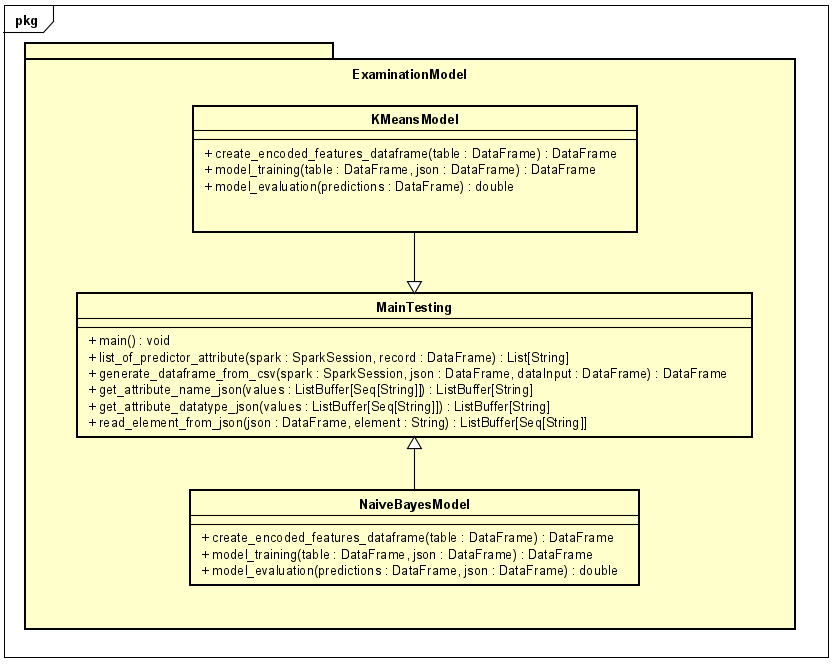
\includegraphics[scale=0.6]{dc_examination_model}
	\caption{Diagram Kelas pada ExaminationModel}
	\label{fig:dc_examination_model}
\end{figure}

\subsubsection{Kelas \textit{KMeansModel}}
Kelas \textit{KMeansModel} merupakan kelas dengan tipe \textit{class}. Hal ini dikarenakan kelas \textit{KMeansModel} berfungsi sebagai model untuk membuat atribut dan method pada objek \textit{KMeansModel}. Kelas \textit{KMeansModel} bertujuan membuat pemodelan \textit{k-means} dan menghitung \textit{silhouette score}.\\

\noindent \noindent Berikut deskripsi method pada kelas \textit{KMeansModel}:

\begin{itemize}

\item \texttt{create\_encoded\_features\_dataframe} dengan parameter \texttt{table(DataFrame)} adalah fungsi yang bertujuan untuk membuat tabel data baru yang berisi nilai aktual, label index, vektor masing-masing atribut, dan vektor dari masing-masing label index.

\item \texttt{model\_training} dengan parameter \texttt{table(DataFrame)}, \texttt{json(DataFrame)} adalah fungsi yang bertujuan untuk membuat model pelatihan k-means dan menghasilkan tabel hasil pengelompokan data berdasarkan input vektor fitur pada setiap baris data.

\item \texttt{model\_evaluation} dengan parameter \texttt{predictions(DataFrame)}adalah fungsi yang bertujuan untuk mencari tahu seberapa baik model k-means yang dibuat dengan menghitung silhouette score. Jika silhouette score mendekati nilai 1, maka hasil pengelompokan sudah baik.

\end{itemize}

\noindent Berikut implementasi method \texttt{model\_training}:

\begin{minipage}{.95\linewidth}
\begin{algorithm}[H]
  \caption{Membuat Pemodelan K-Means}\label{alg:6}
  \begin{algorithmic}[1]
  %-------------- Input & Output -----------------
  \State \textbf{Function} \texttt{model\_training(table,json)}
  \State \textbf{Input:} table data, JSON
  \State \textbf{Output:} table of cluster data.
  \\
  %-------------- Baris 1-3 -----------------
  \State{k = json.select("k\_means.k").first().getLong(0).toInt}
  \State{kmeans = new KMeans().setK(k).setFeaturesCol("features").setPredictionCol("prediction")}
  \State{model = kmeans.fit(table)}
  \State{predictions  = model.transform(table)}
  \State{return predictions} 
  \end{algorithmic}
\end{algorithm}
\end{minipage}

\vspace{0.2cm}
\begin{itemize}
\item Baris 5: baris ini mendapatkan nilai \texttt{k} dari atribut \texttt{k\_means} JSON.
\item Baris 6: baris ini membuat model KMeans menggunakan parameter k pada baris sebelumnya.
\item Baris 7: baris ini melakukan pelatihan model k-means dengan parameter tabel data.
\item Baris 8: baris ini melakukan prediksi model k-means terhadap parameter tabel data.
\end{itemize}

\noindent Berikut implementasi method \texttt{model\_evaluation}:

\begin{minipage}{.8\linewidth}
\begin{algorithm}[H]
  \caption{Menghitung Silhouette Score}\label{alg:6}
  \begin{algorithmic}[1]
  %-------------- Input & Output -----------------
  \State \textbf{Function} \texttt{calculate\_numeric\_distance(num1,num2,max,min)}
  \State \textbf{Input:} numeric 1, numeric 2, maximum number, maximum number.
  \State \textbf{Output:} numeric distance.
  \\
  %-------------- Baris 1-3 -----------------
  \State{evaluator = new ClusteringEvaluator()}
  \State{silhouette\_score = evaluator.evaluate(predictions)}
  \State{return silhouette\_score}
  \end{algorithmic}
\end{algorithm}
\end{minipage}

\vspace{0.2cm}
\begin{itemize}
\item Baris 5: baris ini membuat model ClusteringEvaluator untuk evaluasi k-means.
\item Baris 6: baris ini menghitung nilai \textit{silhouette score} untuk pemodelan k-means.
\end{itemize}

\subsubsection{Kelas \textit{NaiveBayesModel}}
Kelas \textit{NaiveBayesModel} merupakan kelas dengan tipe \textit{class}, karena kelas \textit{NaiveBayesModel} hanya berfungsi sebagai model untuk membuat atribut dan fungsi pada objek \textit{NaiveBayesModel}. Kelas ini bertujuan untuk melakukan pemodelan \textit{naive bayes} dan menghitung \textit{accuracy}.\\

\noindent Berikut deskripsi method pada kelas \textit{NaiveBayesModel}:

\begin{itemize}

\item \texttt{create\_encoded\_features\_dataframe} dengan parameter \texttt{table(DataFrame)} adalah fungsi yang bertujuan untuk membuat tabel data baru yang berisi nilai aktual, label index, vektor untuk masing-masing atribut, dan ditambah satu kolom baru untuk menyimpan vektor fitur dari label index. Output fungsi ini menjadi input pada fungsi \texttt{model\_training}

\item \texttt{model\_training} dengan parameter \texttt{table(DataFrame)}, \texttt{json(DataFrame)} adalah fungsi yang bertujuan untuk membuat model pelatihan naive bayes dan menghasilkan tabel klasifikasi data berdasarkan input vektor fitur untuk setiap baris data.

\item \texttt{model\_evaluation} dengan parameter \texttt{predictions(DataFrame)}, \texttt{json(DataFrame)} adalah fungsi yang bertujuan untuk mencari tahu seberapa baik model naive bayes yang dibuat dengan menghitung accuracy score. Apabila nilainya mendekati 1, maka klasifikasi data yang dibuat dengan model naive bayes sudah mendekati benar.

\end{itemize}

\noindent Berikut implementasi method \texttt{model\_training}:

\begin{minipage}{.8\linewidth}
\begin{algorithm}[H]
  \caption{Membuat Pemodelan Naive Bayes}\label{alg:6}
  \begin{algorithmic}[1]
  %-------------- Input & Output -----------------
  \State \textbf{Function} \texttt{model\_training(table,json)}
  \State \textbf{Input:} table data, JSON
  \State \textbf{Output:} table of classification data.
  \\
  %-------------- Baris 1-3 -----------------
  \State{attrName = json.select("naive\_bayes.label").first().getString(0)}
  \\
  \State{trainingSet = json.select("naive\_bayes.training\_set").first().getDouble(0)}
  \State{testSet = json.select("naive\_bayes.test\_set").first().getDouble(0)}
  \\
  \State{Array(training, test) = table.randomSplit(Array(trainingSet, testSet))}
  \\
  \State{model = new NaiveBayes().setModelType("multinomial")}
  \State{model = model.setLabelCol(attrName+"\_Index").fit(training)}
  \\
  \State{predictions = model.transform(test)}
  \State{return predictions}
  \end{algorithmic}
\end{algorithm}
\end{minipage}

\vspace{0.2cm}
\begin{itemize}
\item Baris 5: baris ini mendapatkan nilai \texttt{label} dari atribut \texttt{naive\_bayes} JSON.
\item Baris 7: baris ini mendapatkan persentase \texttt{training\_set} dari atribut \texttt{naive\_bayes} JSON. 
\item Baris 8: baris ini mendapatkan persentase \texttt{test\_set} dari atribut \texttt{naive\_bayes} JSON. 
\item Baris 10: baris ini membagi data menjadi data training dan data test berdasarkan persentase dari atribut \texttt{trainingSet} dan \texttt{testSet} pada baris sebelumnya.
\item Baris 12: baris ini digunakan untuk membuat model NaiveBayes bertipe "multinomial".
\item Baris 13: baris ini melakukan pelatihan model naive bayes dengan data training.
\item Baris 15: baris ini melakukan prediksi model naive bayes dengan data test.
\end{itemize}

\newpage
\noindent Berikut implementasi method \texttt{model\_evaluation}:

\begin{minipage}{.8\linewidth}
\begin{algorithm}[H]
  \caption{Menghitung Silhouette Score}\label{alg:6}
  \begin{algorithmic}[1]
  %-------------- Input & Output -----------------
  \State \textbf{Function} \texttt{calculate\_numeric\_distance(num1,num2,max,min)}
  \State \textbf{Input:} numeric 1, numeric 2, maximum number, maximum number.
  \State \textbf{Output:} numeric distance.
  \\
  %-------------- Baris 1-3 -----------------
  \State{attrName = json.select("naive\_bayes.label").first().getString(0)}
  \State{evaluator = new MulticlassClassificationEvaluator()}
  \State{evaluator = evaluator.setLabelCol(attrName+"\_Index")}
  \State{evaluator = evaluator.setPredictionCol("prediction")}
  \State{evaluator = evaluator.setMetricName("accuracy")}  
  \State{accuracy = evaluator.evaluate(predictions)}
  \State{return accuracy}
  \end{algorithmic}
\end{algorithm}
\end{minipage}

\vspace{0.2cm}
\begin{itemize}
\item Baris 5: baris ini mendapatkan nilai \texttt{label} dari atribut \texttt{naive\_bayes} JSON.
\item Baris 6-9: baris ini membuat model evaluasi \texttt{MulticlassClassificationEvaluator} untuk mengetahui nilai akurasi dari hasil klasifikasi pemodelan naive bayes.
\item Baris 10: baris ini mengembalikan hasil akurasi untuk pemodelan naive bayes.
\end{itemize}

\subsubsection{Kelas \textit{MainTesting}}
Kelas \textit{MainTesting} merupakan kelas dengan tipe \textit{object}. Hal ini dikarenakan kelas \textit{MainTesting} berperan penting untuk melakukan eksekusi perangkat lunak pengujian terhadap masalah pengelompokan data dengan k-means dan masalah klasifikasi data dengan naive bayes. Kelas ini juga menangani eksekusi evaluasi kedua model tersebut.\\

\noindent Berikut deskripsi method pada kelas \textit{MainTesting}:

\begin{itemize}

\item \texttt{main} adalah fungsi yang bertujuan untuk melakukan proses eksekusi perangkat lunak pengujian dengan membuat objek NaiveBayesModel dan objek KMeansModel.

\item \texttt{list\_of\_predictor\_attribute} dengan parameter \texttt{spark(SparkSession)}, \texttt{record(DataFrame)} adalah fungsi yang bertujuan untuk mendapatkan nilai kolom-kolom prediktor dari tabel data.

\item \texttt{generate\_dataframe\_from\_csv} dengan parameter \texttt{spark(SparkSession)}, \texttt{json(DataFrame)}, \texttt{dataInput(DataFrame)} adalah fungsi yang bertujuan untuk mengambil data \texttt{quasi\_identifier} dan \texttt{sensitive\_attribute} pada JSON. Output dari fungsi ini adalah array 2 dimensi berisi informasi mengenai nama atribut dan kategori atribut (\textit{category/numeric}).

\item \texttt{get\_attribute\_name\_json} dengan parameter \texttt{values(ListBuffer[Seq[String]])} adalah fungsi yang bertujuan untuk mendapatkan nama-nama atribut berdasarkan output array 2 dimensi dari fungsi \texttt{generate\_dataframe\_from\_csv}.

\item \texttt{get\_attribute\_datatype\_json} dengan parameter \texttt{values(ListBuffer[Seq[String]])} adalah fungsi yang bertujuan untuk mengubah atribut dengan tipe "category" menjadi String, sedangkan atribut dengan tipe "numeric" menjadi Integer. 

\item \texttt{read\_element\_from\_json} dengan parameter \texttt{json(DataFrame)}, \texttt{element(String)} adalah fungsi yang bertujuan untuk mendapatkan nilai atribut tertentu pada JSON. Fungsi ini dipanggil pada fungsi lain yaitu \texttt{generate\_dataframe\_from\_csv} untuk mengambil nilai dari atribut \texttt{quasi\_identifier} dan \texttt{sensitive\_identifier}.

\end{itemize}


\section{Masukan Perangkat Lunak}
Perangkat lunak membutuhkan masukan berupa data input .csv yang berisi tabel privat beserta nama atributnya. Pada file .csv, baris pertama merupakan nama atribut dan baris berikutnya merupakan data. Setiap atribut dipisahkan dengan tanda koma (","), sedangkan data baru dipisahkan dengan baris. Format file .csv dapat dilihat pada Listing \ref{lst:pl_csv}.

\begin{lstlisting}[basicstyle=\ttfamily, frame=single,
	columns=fullflexible, keepspaces=true, breaklines=true, label=lst:pl_csv, caption=Dataset Adult]
age,workclass,zip,education,year_of_education,marital_status,occupation
39,State-gov,77516,Bachelors,13,Never-married,Adm-clerical
50,Self-emp-not-inc,83311,Bachelors,13,Married-civ-spouse,Exec-managerial
38,Private,215646,HS-grad,9,Divorced,Handlers-cleaners
53,Private,234721,11th,7,Married-civ-spouse,Handlers-cleaners
\end{lstlisting}

\subsection{Masukan Perangkat Lunak Eksplorasi}
Perangkat lunak ekplorasi membutuhkan data masukan tambahan yaitu file .json yang berisi pohon klasifikasi serta tipe dan jenis atribut. File .json menerapkan format penyimpanan data dengan diawali oleh tanda ("\{ \}") dan diisi oleh nilai \textit{key,value} yang dipisahkan oleh tanda titik dua (":"). Format file .json dapat dilihat pada Listing \ref{lst:eksplor_json}.\\

\noindent Berikut spesifikasi input .json untuk perangkat lunak eksplorasi:

\begin{itemize}

\item \texttt{input\_path} adalah lokasi penyimpanan data input perangkat lunak. Atribut ini akan memberi tahu Spark untuk mengambil data input pada lokasi ini.

\item \texttt{output\_path} adalah lokasi penyimpanan hasil output perangkat lunak. Atribut ini akan memberi tahu Spark untuk menyimpan hasil output pada lokasi ini.

\item \texttt{selected\_column} adalah array yang menyimpan informasi pemilihan atribut. Atribut ini menyimpan 2 jenis informasi penting dalam pemilihan atribut, yaitu

\begin{itemize}

\item \texttt{attrName} adalah nama atribut yang ingin dipilih pada tabel data. Atribut ini akan memberi tahu Spark untuk mengambil atribut berdasarkan nama atribut.

\item \texttt{dataType} adalah jenis tipe data atribut yang telah dipilih. Atribut ini akan memberi tahu Spark untuk menyimpan atribut yang dipilih dalam format tertentu.

\end{itemize}

\end{itemize}

\begin{lstlisting}[basicstyle=\ttfamily, frame=single,
	columns=fullflexible, keepspaces=true, breaklines=true, label=lst:eksplor_json, caption=Input JSON untuk Eksplorasi Data]
{
  "input_path": "<path data input>",
  "output_path": "<path data output>",
  "selected_column": [
      {
        "attrName": "<nama atribut>",
        "dataType": "<tipe data atribut>"
      },
      {
        "attrName": "<nama atribut>",
        "dataType": "<tipe data atribut>"
      }
  ]
}
\end{lstlisting}

\subsection{Masukan Perangkat Lunak Anonimisasi}
Perangkat lunak anonimisasi membutuhkan data masukan tambahan yaitu file .json yang berisi pohon klasifikasi serta tipe dan jenis atribut. File .json menerapkan format penyimpanan data dengan diawali oleh tanda ("\{ \}") dan diisi oleh nilai \textit{key,value} yang dipisahkan oleh tanda titik dua (":"). Format file .json dapat dilihat pada Listing \ref{lst:anon_json}.\\

\noindent Berikut spesifikasi input .json untuk perangkat lunak anonimisasi:

\begin{itemize}
\item \texttt{k} adalah nilai konstanta k-anonymity dan greedy k-member clustering. Atribut ini memiliki tipe data Integer sehingga nilainya harus bilangan bulat.

\item \texttt{num\_sample\_datas} adalah jumlah sample data. Atribut ini memiliki tipe data Integer sehingga nilainya harus dinyatakan dalam bilangan bulat.

\item \texttt{input\_path} adalah lokasi penyimpanan data input perangkat lunak. Atribut ini akan memberi tahu Spark untuk mengambil data input pada lokasi ini.

\item \texttt{output\_path} adalah lokasi penyimpanan hasil output perangkat lunak. Atribut ini akan memberi tahu Spark untuk menyimpan hasil output pada lokasi ini.

\item \texttt{identifiers} adalah array yang berisi nama-nama atribut yang dapat mengungkapkan identitas sebuah data. Atribut ini akan dihilangkan pada tabel anonimisasi.

\item \texttt{sensitive\_identifiers} adalah array yang berisi nama-nama atribut yang nilainya bersifat sensitif. Atribut ini akan tetap ada pada tabel dianonimisasi.

\item \texttt{quasi\_identifiers} adalah atribut yang nilainya dapat dipakai untuk mengungkap entitas data. Atribut ini berisi pasangan nilai berupa nama atribut dan jenis atribut. Jenis atribut diisi dengan nilai "category" untuk menyatakan atribut kategori, sedangkan untuk menyatakan atribut numerik jenis atribut akan diisi dengan nilai "numeric".

\item \texttt{domain\_generalization\_hierarchy} adalah array yang menyimpan informasi mengenai pembentukan pohon DGH. Atribut ini menyimpan 5 jenis informasi penting dalam pembentukan pohon DGH, yaitu:

\begin{itemize}
\item \texttt{attrName} adalah nama atribut yang ingin dipilih pada tabel data. Atribut ini akan memberi tahu Spark untuk mengambil atribut berdasarkan nama atribut.

\item \texttt{value} adalah nilai-nilai yang mungkin muncul untuk atribut yang terpilih. Atribut ini akan digunakan untuk memberi nama pada sebuah node di pohon DGH.

\item \texttt{parent} adalah nilai yang menyatakan nama dari sebuah node root. Atribut ini akan digunakan untuk menyatakan parent dari sebuah node di pohon DGH.

\item \texttt{level} adalah nilai yang menyatakan ketinggian node di pohon DGH. Atribut ini digunakan untuk menempatkan node di ketinggian tertentu di pohon DGH.

\item \texttt{position} adalah nilai yang menyatakan posisi node di pohon DGH. Atribut ini digunakan untuk menempatkan node di posisi (kiri/kanan) dari node parent.
\end{itemize}

\end{itemize}

\noindent Berikut adalah hal penting yang perlu diperhatikan terkait input (.json):

\begin{itemize}

\item Nilai atribut yang dicantumkan pada \texttt{domain\_generalization\_hierarchy} di salah satu atribut harus mencakup seluruh kemungkinan nilai untuk atribut tersebut. Apabila tidak terpenuhi, maka beberapa nilai tidak dapat dianonimisasi.

\item Semakin banyak atribut yang dicantumkan pada \texttt{quasi\_identifier}, maka waktu komputasi akan semakin lama untuk dijalankan pada komputer lokal.

\end{itemize}




\newpage
\begin{lstlisting}[basicstyle=\ttfamily, frame=single,
	columns=fullflexible, keepspaces=true, breaklines=true, label=lst:anon_json, caption=Input JSON untuk Anonimisasi Data]
{
  "k": <konstanta untuk k-anonymity dan greedy k-member clustering>,
  "num_sample_datas": <jumlah sampel data>,
  "input_path": "<path data input>",
  "output_path": "<path data output>",
  "identifier": [
      {
        "attrName": "<nama atribut>",
        "dataType": "<tipe data atribut>"
      }
  ],
  "sensitive_identifier": [
      {
        "attrName": "<nama atribut>",
        "dataType": "<jenis atribut>"
      }
  ],
  "quasi_identifier": [
      {
        "attrName": "<nama atribut>",
        "dataType": "<jenis atribut>"
      },
      {
        "attrName": "<nama atribut>",
        "dataType": "<jenis atribut>"
      }
  ],
  "domain_generalization_hierarchy": {
      "<nama atribut>":[
          {
            "value": "<nilai atribut>",
            "parent": "<nilai atribut parent>",
            "level": "1",
            "position": "null"
          },
          {
            "value": "<nilai atribut>",
            "parent": "<nilai atribut parent>",
            "level": "2",
            "position": "left"
          },
          {
            "value": "<nilai atribut>",
            "parent": "<nilai atribut parent>",
            "level": "2",
            "position": "right"
          }
      ] 
  }
}
\end{lstlisting}


\subsection{Masukan Perangkat Lunak Pengujian}
Perangkat lunak anonimisasi membutuhkan data masukan tambahan yaitu file .json yang berisi pohon klasifikasi serta tipe dan jenis atribut. File .json menerapkan format penyimpanan data dengan diawali oleh tanda ("\{ \}") dan diisi oleh nilai \textit{key,value} yang dipisahkan oleh tanda titik dua (":"). Format file .json dapat dilihat pada Listing \ref{lst:pengujian_json}.\\

\noindent Berikut spesifikasi input .json untuk perangkat lunak pengujian:

\begin{itemize}

\item \texttt{input\_path} adalah lokasi penyimpanan data input perangkat lunak. Atribut ini akan memberi tahu Spark untuk mengambil data input pada lokasi ini.

\item \texttt{output\_path} adalah lokasi penyimpanan hasil output perangkat lunak. Atribut ini akan memberi tahu Spark untuk menyimpan hasil output pada lokasi ini.

\item \texttt{model\_name} adalah jenis model yang akan dipakai untuk pengujian. Atribut ini terdiri dari 2 jenis nilai yaitu \texttt{k\_means,naive\_bayes}.

\item \texttt{selected\_column} adalah array yang menyimpan informasi pemilihan atribut. Atribut ini menyimpan 2 jenis informasi penting dalam pemilihan atribut, yaitu:

\begin{itemize}

\item \texttt{attrName} adalah nama atribut yang ingin dipilih pada tabel data. Atribut ini akan memberi tahu Spark untuk mengambil kolom berdasarkan nama atribut.

\item \texttt{dataType} adalah jenis tipe data atribut yang telah dipilih. Atribut ini akan memberi tahu Spark untuk menyimpan atribut yang dipilih dalam format tertentu.

\end{itemize}

\item \texttt{k\_means} adalah parameter untuk pemodelan k-means. Atribut ini terdiri dari 1 parameter untuk pemodelan k-means, yaitu:

\begin{itemize}

\item \texttt{k} adalah konstanta k pada pemodelan k-means. Atribut ini digunakan untuk menentukan jumlah kelompok data yang ingin dibentuk.

\end{itemize}

\item \texttt{naive\_bayes} adalah parameter untuk pemodelan naive bayes. Atribut ini terdiri dari 3 parameter untuk pemodelan naive bayes, yaitu:

\begin{itemize}

\item \texttt{label} adalah nama atribut yang akan dianggap sebagai label untuk pemodelan naive bayes. Atribut ini digunakan untuk mengklasifikasikan data berdasarkan nilai pada atribut label.

\item \texttt{training\_set} adalah persentase pembagian data training. Umumnya, persentase yang dipilih untuk pembagian data training adalah 0.7.

\item \texttt{test\_set} adalah persentase pembagian data test. Umumnya, persentase yang dipilih untuk pembagian data test adalah 0.3.

\end{itemize}


\end{itemize}

\noindent Berikut adalah hal penting yang perlu diperhatikan terkait input (.json):

\begin{itemize}

\item Atribut \texttt{input\_path} untuk dapat diisi menggunakan lokasi data setelah anonimisasi maupun data sebelum anonimisasi untuk membandingkan hasil keduanya.
\item Atribut \texttt{model\_name} hanya boleh diisi oleh satu jenis model, tidak boleh lebih. Jika diisi lebih dari satu nilai, maka program akan mengeluarkan pesan error.
\item Atribut \texttt{training\_set} dan \texttt{test\_set} harus berada pada rentang 0 sampai dengan 1. Lalu ketika dijumlah \texttt{training\_set} dan \texttt{test\_set} harus benilai 1.

\end{itemize}

\newpage
\begin{lstlisting}[basicstyle=\ttfamily, frame=single,
	columns=fullflexible, keepspaces=true, breaklines=true, label=pengujian_json, caption=Input JSON untuk Pengujian Data]
{
  "input_path": "<path data input>",
  "output_path": "<path data output>",
  "model_name": "<model pengujian (k_means/naive_bayes)>",
  "selected_column": [
      {
        "attrName": "<nama atribut>",
        "dataType": "<jenis atribut>"
      },
      {
        "attrName": "<nama atribut>",
        "dataType": "<jenis atribut>"
      }
  ],
  "k_means": {
      "k": <nilai k untuk k_means>
  },
  "naive_bayes": {
      "label": "<nama atribut>",
      "training_set": <persentase training_set (0.7)>,
      "test_set": <persentase training_set (0.3)>
  }
}
\end{lstlisting}




